\documentclass[12pt,letterpaper]{article}
\usepackage[letterpaper,left=0.62in,right=0.62in,top=0.75in,bottom=0.65in,headheight=14pt,headsep=0.17in,footskip=0.32in]{geometry}
\usepackage[T1]{fontenc}
\usepackage{lmodern}
\pdfmapfile{+lm.map}
\usepackage{tikz}
\usepackage{fancyhdr}
\definecolor{Rfill}{RGB}{251,227,225}
\definecolor{Bfill}{RGB}{223,235,251}
\definecolor{Yfill}{RGB}{255,247,203}
\pagestyle{fancy}
\fancyhf{}
\renewcommand{\headrulewidth}{0pt}
\renewcommand{\footrulewidth}{0pt}
\setlength{\parindent}{0pt}
\setlength{\parskip}{0pt}
\setlength{\emergencystretch}{2em}
\raggedbottom
\sffamily
\fancyhead[L]{\fontsize{10.5}{12}\selectfont Week 16 / Three-color triangles / Grades 4--5}
\fancyfoot[L]{\fontsize{9}{11}\selectfont Bellingham Math Circle / Week 16 / F16-45-v2}
\fancyfoot[R]{\fontsize{9}{11}\selectfont\thepage}
\begin{document}
\fontsize{12.5}{16.5}\selectfont
Write R, B, or Y on every empty dot. Keep the printed letters. Each outside side allows only the letters beside it. A little triangle has no lines inside.\par\vspace{0.23in}
\textbf{Problem 1:} Find a filling with as few little triangles containing R, B, and Y as you can, and another with as many as you can. Which counts between your two records can you make?\par\vspace{0.16in}
\begin{center}
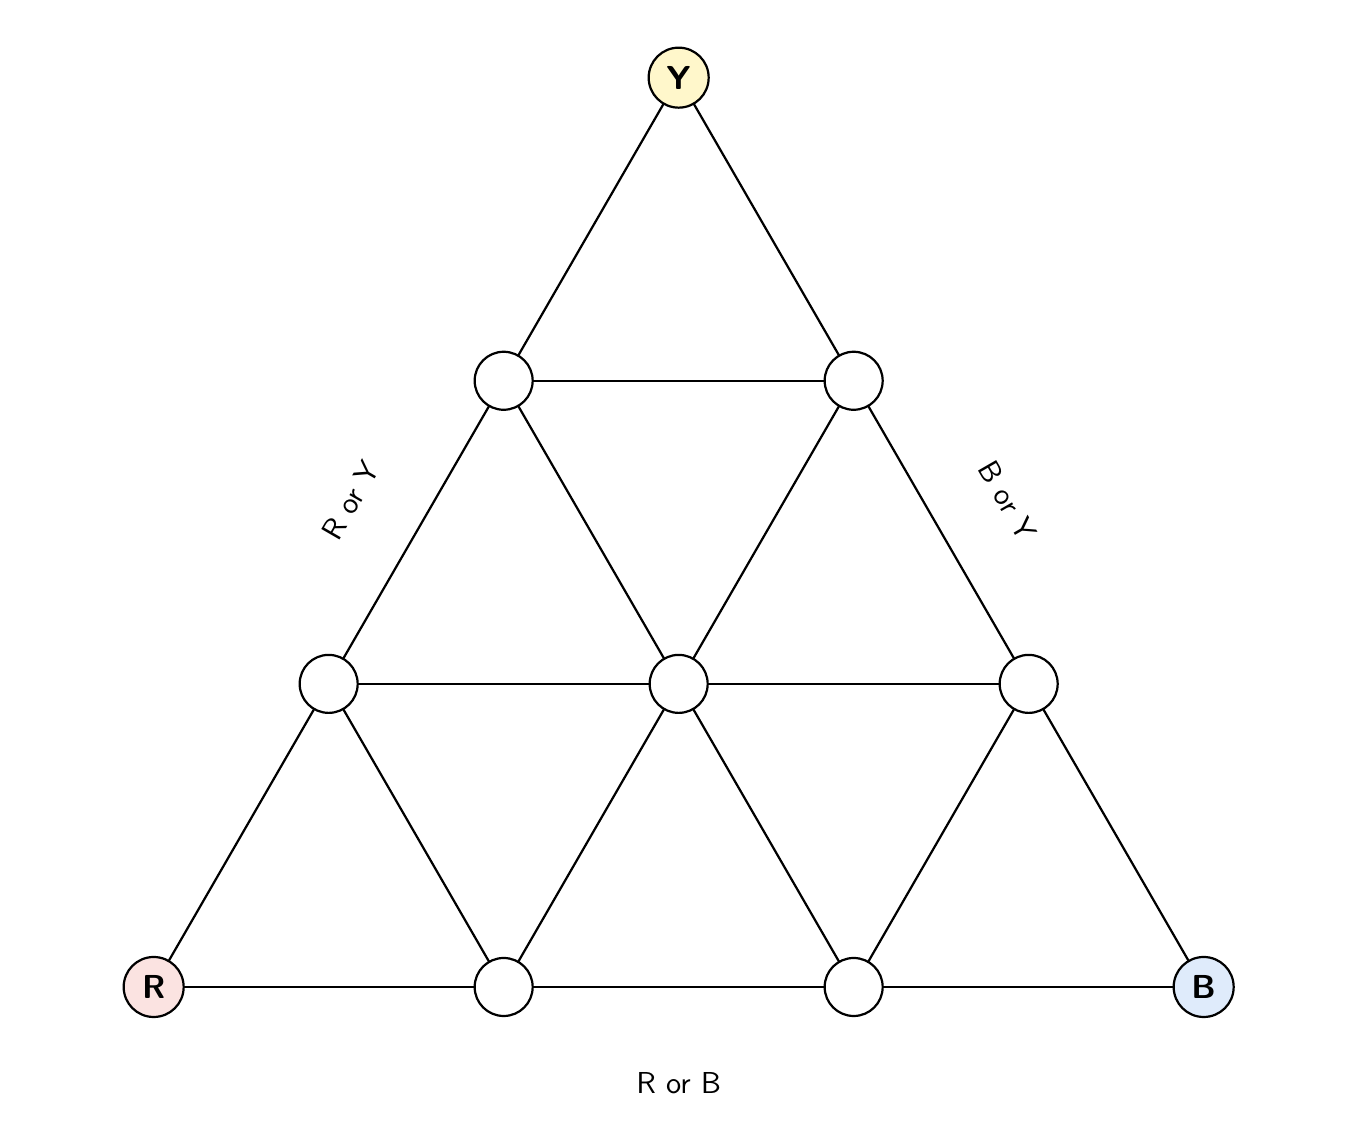
\begin{tikzpicture}[x=1in,y=1in,line cap=round,line join=round]
\path[use as bounding box] (-0.63,-0.64) rectangle (5.8800,4.7966);
\draw[line width=0.8pt] (0.0000,0.0000) -- (0.8750,1.5155);
\draw[line width=0.8pt] (0.0000,0.0000) -- (1.7500,0.0000);
\draw[line width=0.8pt] (0.8750,1.5155) -- (1.7500,3.0311);
\draw[line width=0.8pt] (0.8750,1.5155) -- (1.7500,0.0000);
\draw[line width=0.8pt] (0.8750,1.5155) -- (2.6250,1.5155);
\draw[line width=0.8pt] (1.7500,3.0311) -- (2.6250,4.5466);
\draw[line width=0.8pt] (1.7500,3.0311) -- (2.6250,1.5155);
\draw[line width=0.8pt] (1.7500,3.0311) -- (3.5000,3.0311);
\draw[line width=0.8pt] (2.6250,4.5466) -- (3.5000,3.0311);
\draw[line width=0.8pt] (1.7500,0.0000) -- (2.6250,1.5155);
\draw[line width=0.8pt] (1.7500,0.0000) -- (3.5000,0.0000);
\draw[line width=0.8pt] (2.6250,1.5155) -- (3.5000,3.0311);
\draw[line width=0.8pt] (2.6250,1.5155) -- (3.5000,0.0000);
\draw[line width=0.8pt] (2.6250,1.5155) -- (4.3750,1.5155);
\draw[line width=0.8pt] (3.5000,3.0311) -- (4.3750,1.5155);
\draw[line width=0.8pt] (3.5000,0.0000) -- (4.3750,1.5155);
\draw[line width=0.8pt] (3.5000,0.0000) -- (5.2500,0.0000);
\draw[line width=0.8pt] (4.3750,1.5155) -- (5.2500,0.0000);
\node[circle,draw,line width=0.8pt,fill=Rfill,minimum size=0.30in,inner sep=0pt,font=\sffamily\bfseries\fontsize{11.5}{12}\selectfont] at (0.0000,0.0000) {R};
\draw[line width=0.8pt,fill=white] (1.7500,0.0000) circle[radius=0.145in];
\draw[line width=0.8pt,fill=white] (3.5000,0.0000) circle[radius=0.145in];
\node[circle,draw,line width=0.8pt,fill=Bfill,minimum size=0.30in,inner sep=0pt,font=\sffamily\bfseries\fontsize{11.5}{12}\selectfont] at (5.2500,0.0000) {B};
\draw[line width=0.8pt,fill=white] (0.8750,1.5155) circle[radius=0.145in];
\draw[line width=0.8pt,fill=white] (2.6250,1.5155) circle[radius=0.145in];
\draw[line width=0.8pt,fill=white] (4.3750,1.5155) circle[radius=0.145in];
\draw[line width=0.8pt,fill=white] (1.7500,3.0311) circle[radius=0.145in];
\draw[line width=0.8pt,fill=white] (3.5000,3.0311) circle[radius=0.145in];
\node[circle,draw,line width=0.8pt,fill=Yfill,minimum size=0.30in,inner sep=0pt,font=\sffamily\bfseries\fontsize{11.5}{12}\selectfont] at (2.6250,4.5466) {Y};
\node[rotate=60,font=\sffamily\fontsize{11}{12}\selectfont] at (0.9825,2.4333) {R or Y};
\node[rotate=-60,font=\sffamily\fontsize{11}{12}\selectfont] at (4.2675,2.4333) {B or Y};
\node[font=\sffamily\fontsize{11}{12}\selectfont] at (2.6250,-0.48) {R or B};
\end{tikzpicture}
\end{center}
\newpage
\textbf{Problem 1:} Find a filling with as few little triangles containing R, B, and Y as you can, and another with as many as you can. Which counts between your two records can you make?\par\vspace{0.16in}
\begin{center}
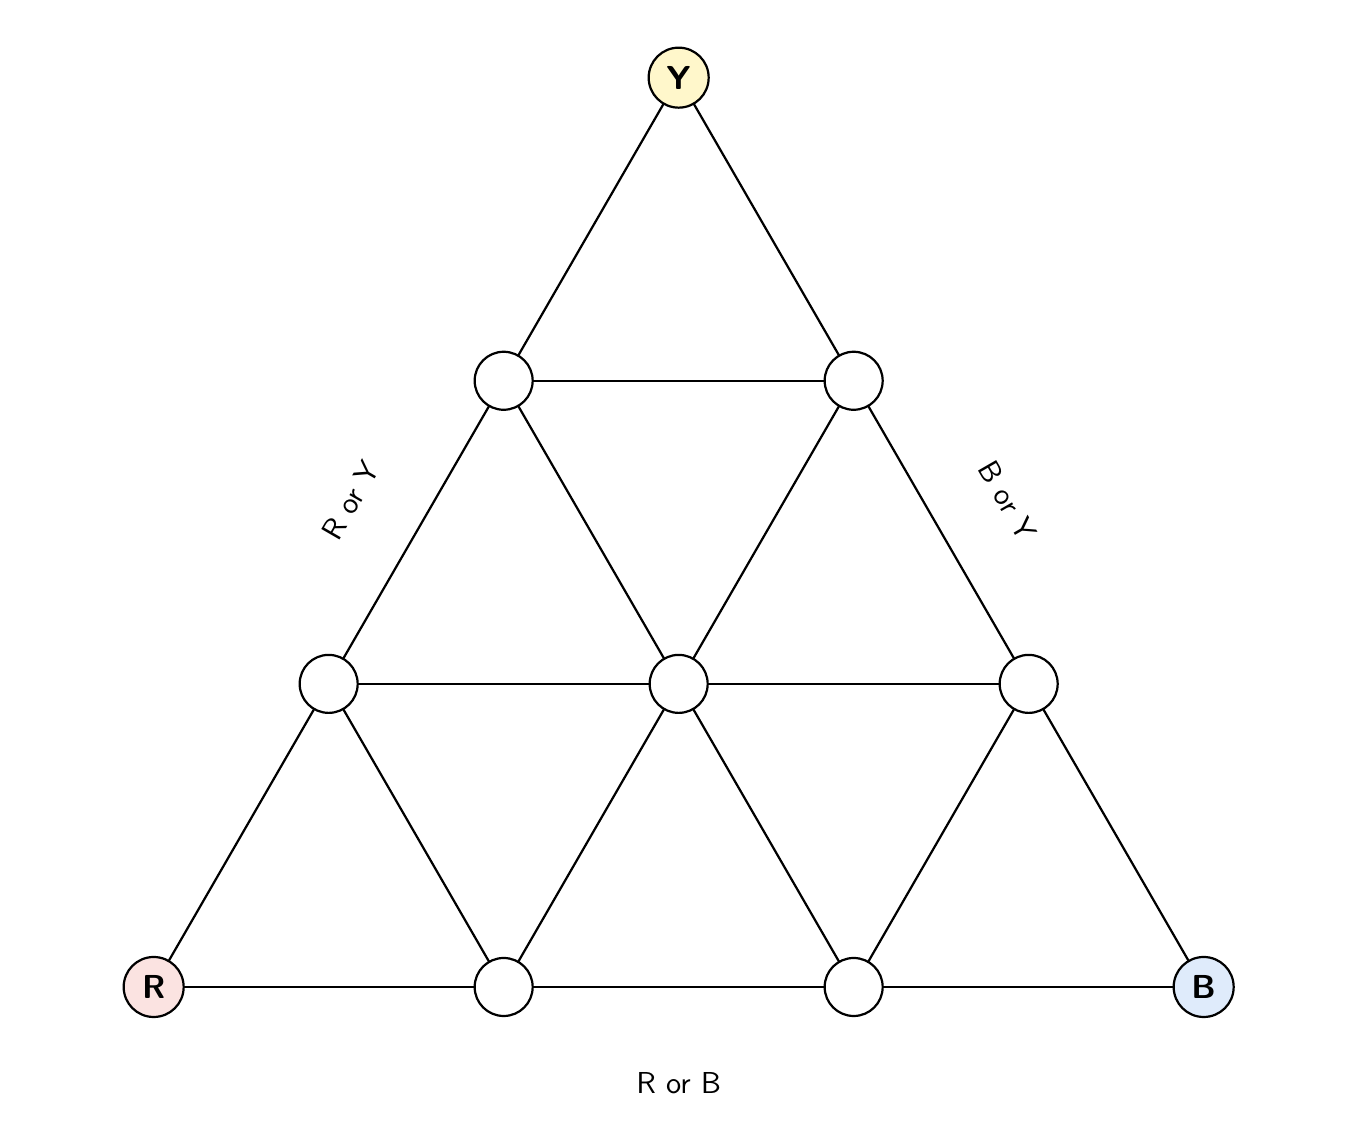
\begin{tikzpicture}[x=1in,y=1in,line cap=round,line join=round]
\path[use as bounding box] (-0.63,-0.64) rectangle (5.8800,4.7966);
\draw[line width=0.8pt] (0.0000,0.0000) -- (0.8750,1.5155);
\draw[line width=0.8pt] (0.0000,0.0000) -- (1.7500,0.0000);
\draw[line width=0.8pt] (0.8750,1.5155) -- (1.7500,3.0311);
\draw[line width=0.8pt] (0.8750,1.5155) -- (1.7500,0.0000);
\draw[line width=0.8pt] (0.8750,1.5155) -- (2.6250,1.5155);
\draw[line width=0.8pt] (1.7500,3.0311) -- (2.6250,4.5466);
\draw[line width=0.8pt] (1.7500,3.0311) -- (2.6250,1.5155);
\draw[line width=0.8pt] (1.7500,3.0311) -- (3.5000,3.0311);
\draw[line width=0.8pt] (2.6250,4.5466) -- (3.5000,3.0311);
\draw[line width=0.8pt] (1.7500,0.0000) -- (2.6250,1.5155);
\draw[line width=0.8pt] (1.7500,0.0000) -- (3.5000,0.0000);
\draw[line width=0.8pt] (2.6250,1.5155) -- (3.5000,3.0311);
\draw[line width=0.8pt] (2.6250,1.5155) -- (3.5000,0.0000);
\draw[line width=0.8pt] (2.6250,1.5155) -- (4.3750,1.5155);
\draw[line width=0.8pt] (3.5000,3.0311) -- (4.3750,1.5155);
\draw[line width=0.8pt] (3.5000,0.0000) -- (4.3750,1.5155);
\draw[line width=0.8pt] (3.5000,0.0000) -- (5.2500,0.0000);
\draw[line width=0.8pt] (4.3750,1.5155) -- (5.2500,0.0000);
\node[circle,draw,line width=0.8pt,fill=Rfill,minimum size=0.30in,inner sep=0pt,font=\sffamily\bfseries\fontsize{11.5}{12}\selectfont] at (0.0000,0.0000) {R};
\draw[line width=0.8pt,fill=white] (1.7500,0.0000) circle[radius=0.145in];
\draw[line width=0.8pt,fill=white] (3.5000,0.0000) circle[radius=0.145in];
\node[circle,draw,line width=0.8pt,fill=Bfill,minimum size=0.30in,inner sep=0pt,font=\sffamily\bfseries\fontsize{11.5}{12}\selectfont] at (5.2500,0.0000) {B};
\draw[line width=0.8pt,fill=white] (0.8750,1.5155) circle[radius=0.145in];
\draw[line width=0.8pt,fill=white] (2.6250,1.5155) circle[radius=0.145in];
\draw[line width=0.8pt,fill=white] (4.3750,1.5155) circle[radius=0.145in];
\draw[line width=0.8pt,fill=white] (1.7500,3.0311) circle[radius=0.145in];
\draw[line width=0.8pt,fill=white] (3.5000,3.0311) circle[radius=0.145in];
\node[circle,draw,line width=0.8pt,fill=Yfill,minimum size=0.30in,inner sep=0pt,font=\sffamily\bfseries\fontsize{11.5}{12}\selectfont] at (2.6250,4.5466) {Y};
\node[rotate=60,font=\sffamily\fontsize{11}{12}\selectfont] at (0.9825,2.4333) {R or Y};
\node[rotate=-60,font=\sffamily\fontsize{11}{12}\selectfont] at (4.2675,2.4333) {B or Y};
\node[font=\sffamily\fontsize{11}{12}\selectfont] at (2.6250,-0.48) {R or B};
\end{tikzpicture}
\end{center}
\newpage
\textbf{Problem 2:} Call an edge with R at one end and B at the other a door. Mark every door. A route crosses through doors and uses no door twice. In a two-door triangle it must use both doors. Draw all the routes, including any that stay inside the big triangle. Can every route from outside return outside?\par\vspace{0.16in}
\begin{center}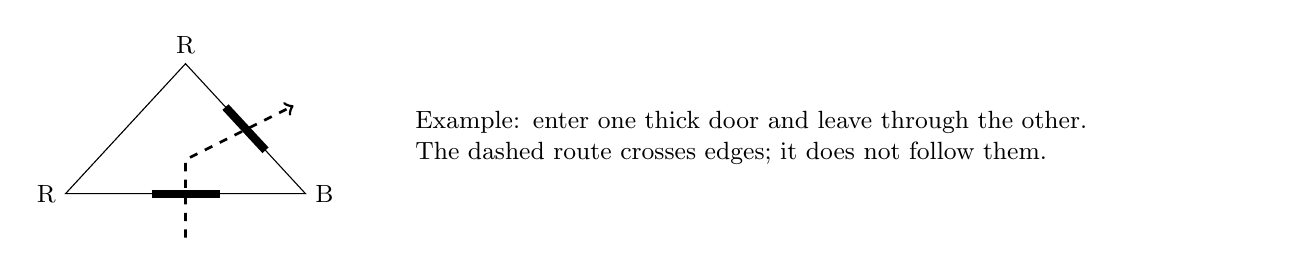
\begin{tikzpicture}[x=1in,y=1in]
\draw (0,0)--(1.2,0)--(.6,.65)--cycle;
\draw[line width=3pt] (.43,0)--(.77,0);
\draw[line width=3pt] (.80,.433)--(1.00,.217);
\node[left,font=\small] at (0,0){R};\node[right,font=\small] at (1.2,0){B};\node[above,font=\small] at (.6,.65){R};
\draw[->,dashed,line width=1pt] (.6,-.22)--(.6,.17)--(1.14,.44);
\node[anchor=west,align=left,text width=4.3in,font=\small] at (1.7,.28){Example: enter one thick door and leave through the other.\\The dashed route crosses edges; it does not follow them.};
\end{tikzpicture}\end{center}
\begin{center}
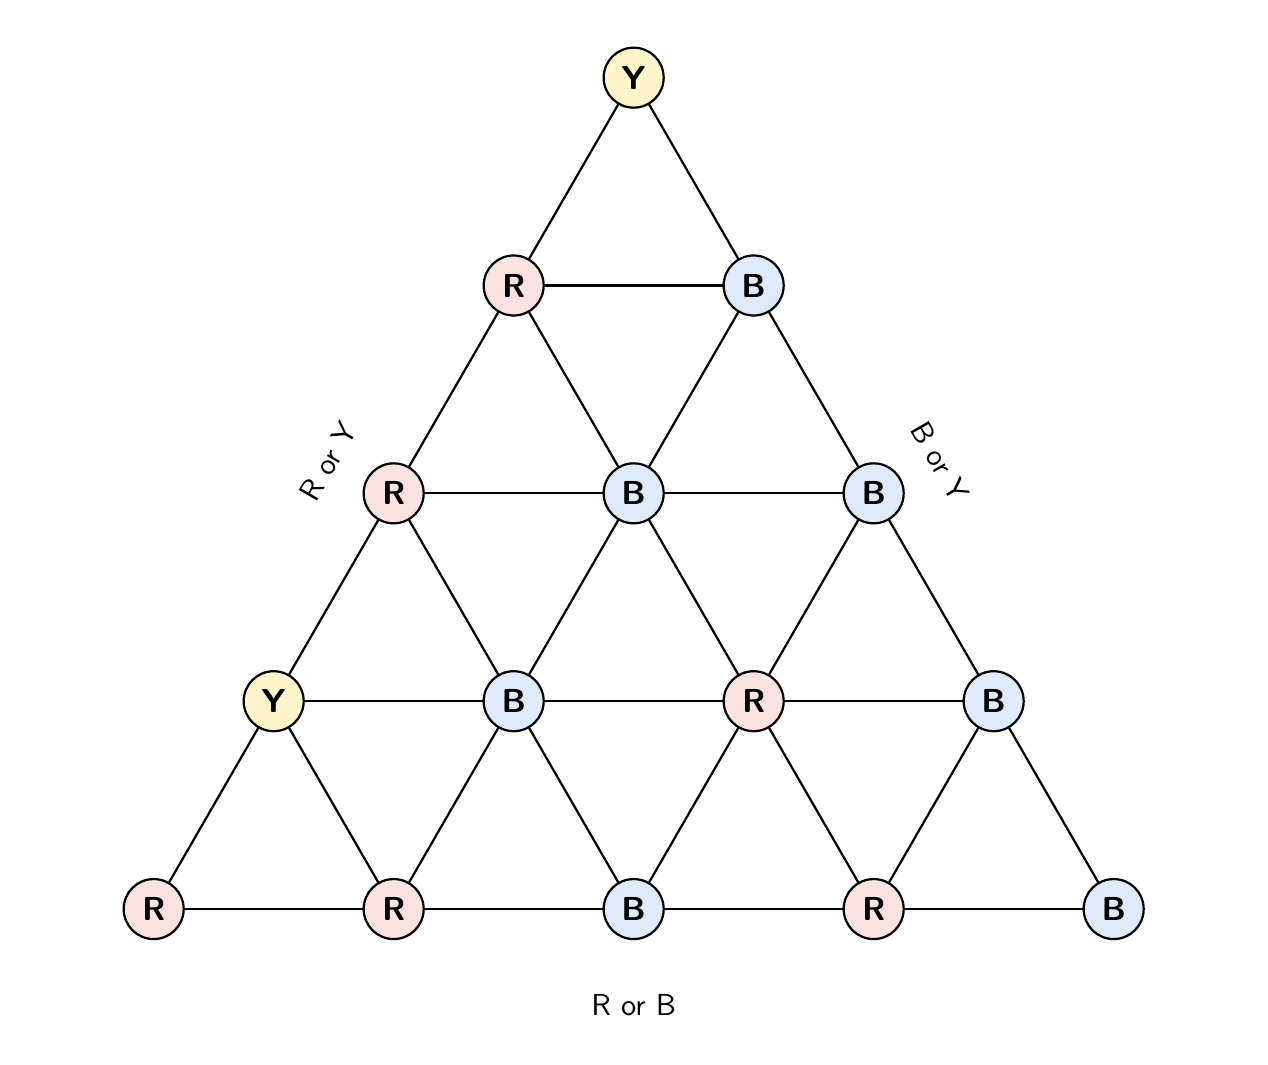
\begin{tikzpicture}[x=1in,y=1in,line cap=round,line join=round]
\path[use as bounding box] (-0.63,-0.64) rectangle (5.4300,4.4069);
\draw[line width=0.8pt] (0.0000,0.0000) -- (0.6000,1.0392);
\draw[line width=0.8pt] (0.0000,0.0000) -- (1.2000,0.0000);
\draw[line width=0.8pt] (0.6000,1.0392) -- (1.2000,2.0785);
\draw[line width=0.8pt] (0.6000,1.0392) -- (1.2000,0.0000);
\draw[line width=0.8pt] (0.6000,1.0392) -- (1.8000,1.0392);
\draw[line width=0.8pt] (1.2000,2.0785) -- (1.8000,3.1177);
\draw[line width=0.8pt] (1.2000,2.0785) -- (1.8000,1.0392);
\draw[line width=0.8pt] (1.2000,2.0785) -- (2.4000,2.0785);
\draw[line width=0.8pt] (1.8000,3.1177) -- (2.4000,4.1569);
\draw[line width=0.8pt] (1.8000,3.1177) -- (2.4000,2.0785);
\draw[line width=0.8pt] (1.8000,3.1177) -- (3.0000,3.1177);
\draw[line width=0.8pt] (2.4000,4.1569) -- (3.0000,3.1177);
\draw[line width=0.8pt] (1.2000,0.0000) -- (1.8000,1.0392);
\draw[line width=0.8pt] (1.2000,0.0000) -- (2.4000,0.0000);
\draw[line width=0.8pt] (1.8000,1.0392) -- (2.4000,2.0785);
\draw[line width=0.8pt] (1.8000,1.0392) -- (2.4000,0.0000);
\draw[line width=0.8pt] (1.8000,1.0392) -- (3.0000,1.0392);
\draw[line width=0.8pt] (2.4000,2.0785) -- (3.0000,3.1177);
\draw[line width=0.8pt] (2.4000,2.0785) -- (3.0000,1.0392);
\draw[line width=0.8pt] (2.4000,2.0785) -- (3.6000,2.0785);
\draw[line width=0.8pt] (3.0000,3.1177) -- (3.6000,2.0785);
\draw[line width=0.8pt] (2.4000,0.0000) -- (3.0000,1.0392);
\draw[line width=0.8pt] (2.4000,0.0000) -- (3.6000,0.0000);
\draw[line width=0.8pt] (3.0000,1.0392) -- (3.6000,2.0785);
\draw[line width=0.8pt] (3.0000,1.0392) -- (3.6000,0.0000);
\draw[line width=0.8pt] (3.0000,1.0392) -- (4.2000,1.0392);
\draw[line width=0.8pt] (3.6000,2.0785) -- (4.2000,1.0392);
\draw[line width=0.8pt] (3.6000,0.0000) -- (4.2000,1.0392);
\draw[line width=0.8pt] (3.6000,0.0000) -- (4.8000,0.0000);
\draw[line width=0.8pt] (4.2000,1.0392) -- (4.8000,0.0000);
\node[circle,draw,line width=0.8pt,fill=Rfill,minimum size=0.30in,inner sep=0pt,font=\sffamily\bfseries\fontsize{11.5}{12}\selectfont] at (0.0000,0.0000) {R};
\node[circle,draw,line width=0.8pt,fill=Rfill,minimum size=0.30in,inner sep=0pt,font=\sffamily\bfseries\fontsize{11.5}{12}\selectfont] at (1.2000,0.0000) {R};
\node[circle,draw,line width=0.8pt,fill=Bfill,minimum size=0.30in,inner sep=0pt,font=\sffamily\bfseries\fontsize{11.5}{12}\selectfont] at (2.4000,0.0000) {B};
\node[circle,draw,line width=0.8pt,fill=Rfill,minimum size=0.30in,inner sep=0pt,font=\sffamily\bfseries\fontsize{11.5}{12}\selectfont] at (3.6000,0.0000) {R};
\node[circle,draw,line width=0.8pt,fill=Bfill,minimum size=0.30in,inner sep=0pt,font=\sffamily\bfseries\fontsize{11.5}{12}\selectfont] at (4.8000,0.0000) {B};
\node[circle,draw,line width=0.8pt,fill=Yfill,minimum size=0.30in,inner sep=0pt,font=\sffamily\bfseries\fontsize{11.5}{12}\selectfont] at (0.6000,1.0392) {Y};
\node[circle,draw,line width=0.8pt,fill=Bfill,minimum size=0.30in,inner sep=0pt,font=\sffamily\bfseries\fontsize{11.5}{12}\selectfont] at (1.8000,1.0392) {B};
\node[circle,draw,line width=0.8pt,fill=Rfill,minimum size=0.30in,inner sep=0pt,font=\sffamily\bfseries\fontsize{11.5}{12}\selectfont] at (3.0000,1.0392) {R};
\node[circle,draw,line width=0.8pt,fill=Bfill,minimum size=0.30in,inner sep=0pt,font=\sffamily\bfseries\fontsize{11.5}{12}\selectfont] at (4.2000,1.0392) {B};
\node[circle,draw,line width=0.8pt,fill=Rfill,minimum size=0.30in,inner sep=0pt,font=\sffamily\bfseries\fontsize{11.5}{12}\selectfont] at (1.2000,2.0785) {R};
\node[circle,draw,line width=0.8pt,fill=Bfill,minimum size=0.30in,inner sep=0pt,font=\sffamily\bfseries\fontsize{11.5}{12}\selectfont] at (2.4000,2.0785) {B};
\node[circle,draw,line width=0.8pt,fill=Bfill,minimum size=0.30in,inner sep=0pt,font=\sffamily\bfseries\fontsize{11.5}{12}\selectfont] at (3.6000,2.0785) {B};
\node[circle,draw,line width=0.8pt,fill=Rfill,minimum size=0.30in,inner sep=0pt,font=\sffamily\bfseries\fontsize{11.5}{12}\selectfont] at (1.8000,3.1177) {R};
\node[circle,draw,line width=0.8pt,fill=Bfill,minimum size=0.30in,inner sep=0pt,font=\sffamily\bfseries\fontsize{11.5}{12}\selectfont] at (3.0000,3.1177) {B};
\node[circle,draw,line width=0.8pt,fill=Yfill,minimum size=0.30in,inner sep=0pt,font=\sffamily\bfseries\fontsize{11.5}{12}\selectfont] at (2.4000,4.1569) {Y};
\node[rotate=60,font=\sffamily\fontsize{11}{12}\selectfont] at (0.8700,2.2385) {R or Y};
\node[rotate=-60,font=\sffamily\fontsize{11}{12}\selectfont] at (3.9300,2.2385) {B or Y};
\node[font=\sffamily\fontsize{11}{12}\selectfont] at (2.4000,-0.48) {R or B};
\end{tikzpicture}
\end{center}
\newpage
\textbf{Problem 3:} Put R, B, or Y on each dot. Find every different filling, counting turns and flips as the same. Record the number of doors in each filling. Which fillings have exactly one door? Could a triangle have three doors?\par\vspace{0.16in}
\begin{center}
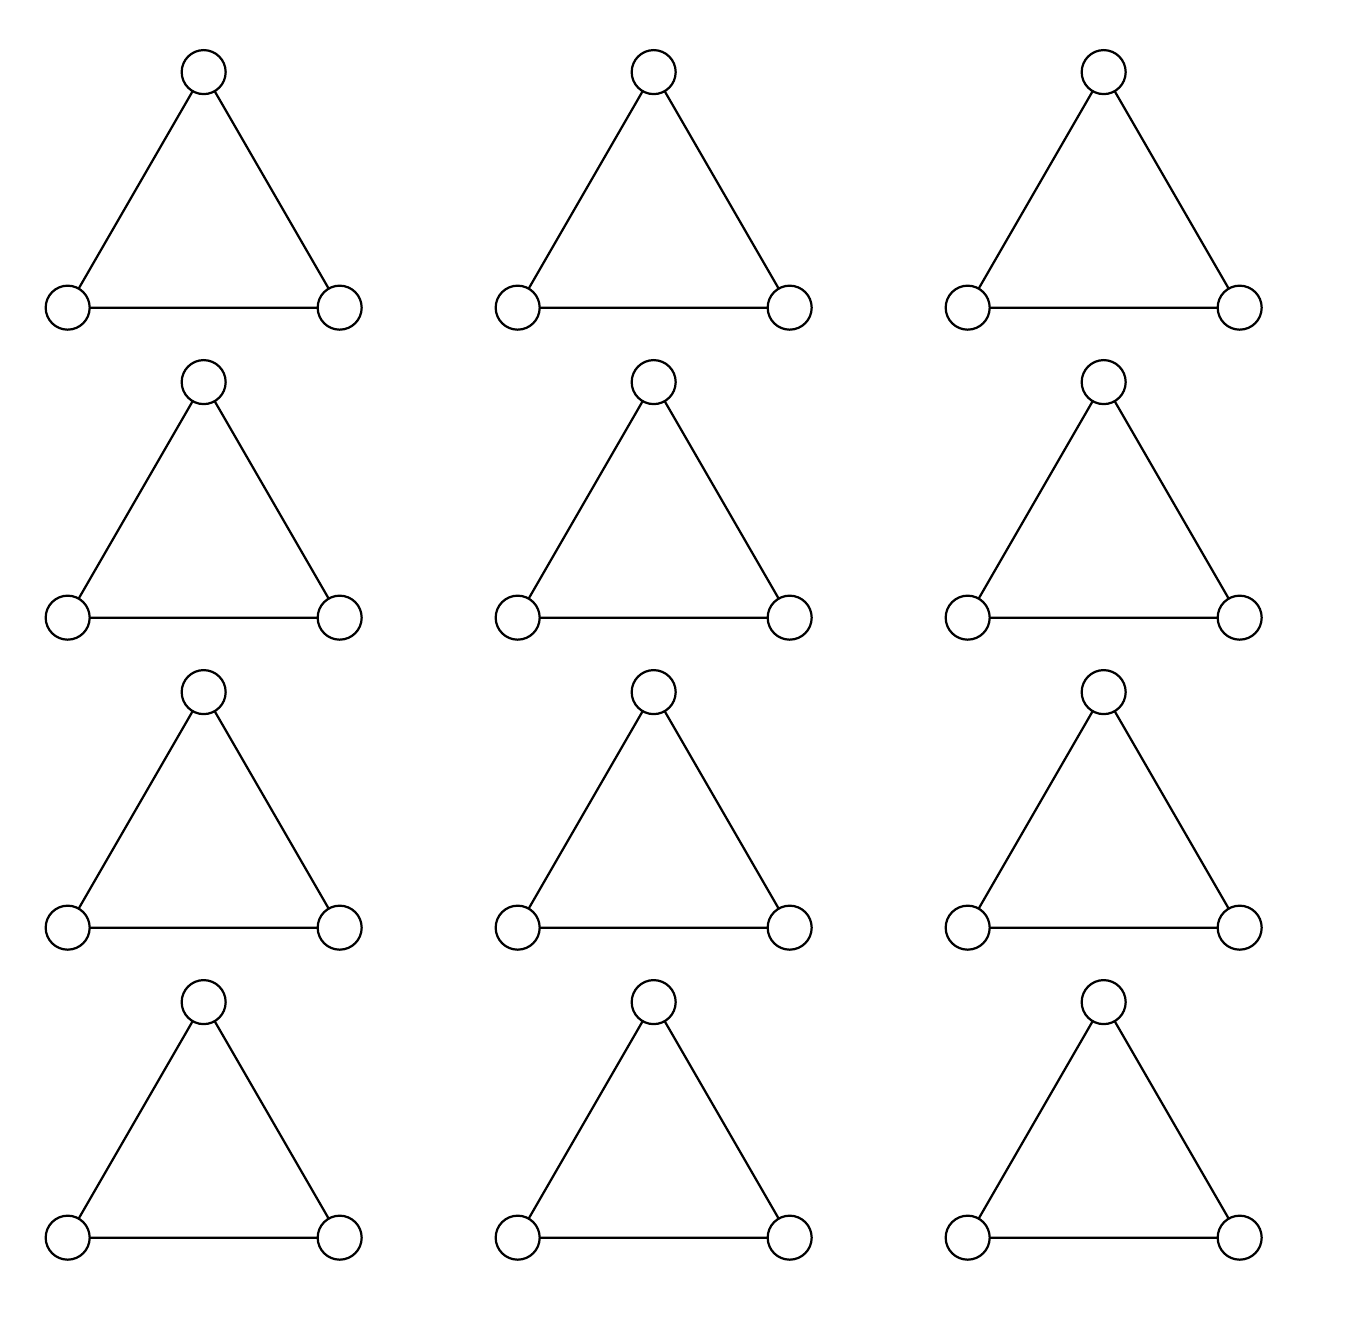
\begin{tikzpicture}[x=1in,y=1in,line cap=round]
\path[use as bounding box] (-0.2,-0.35) rectangle (6.3,6.05);
\draw[line width=0.8pt] (0.0000,4.6500) -- (1.3600,4.6500) -- (0.6800,5.8278) -- cycle;
\draw[line width=0.8pt,fill=white] (0.0000,4.6500) circle[radius=0.11in];
\draw[line width=0.8pt,fill=white] (1.3600,4.6500) circle[radius=0.11in];
\draw[line width=0.8pt,fill=white] (0.6800,5.8278) circle[radius=0.11in];
\draw[line width=0.8pt] (2.2500,4.6500) -- (3.6100,4.6500) -- (2.9300,5.8278) -- cycle;
\draw[line width=0.8pt,fill=white] (2.2500,4.6500) circle[radius=0.11in];
\draw[line width=0.8pt,fill=white] (3.6100,4.6500) circle[radius=0.11in];
\draw[line width=0.8pt,fill=white] (2.9300,5.8278) circle[radius=0.11in];
\draw[line width=0.8pt] (4.5000,4.6500) -- (5.8600,4.6500) -- (5.1800,5.8278) -- cycle;
\draw[line width=0.8pt,fill=white] (4.5000,4.6500) circle[radius=0.11in];
\draw[line width=0.8pt,fill=white] (5.8600,4.6500) circle[radius=0.11in];
\draw[line width=0.8pt,fill=white] (5.1800,5.8278) circle[radius=0.11in];
\draw[line width=0.8pt] (0.0000,3.1000) -- (1.3600,3.1000) -- (0.6800,4.2778) -- cycle;
\draw[line width=0.8pt,fill=white] (0.0000,3.1000) circle[radius=0.11in];
\draw[line width=0.8pt,fill=white] (1.3600,3.1000) circle[radius=0.11in];
\draw[line width=0.8pt,fill=white] (0.6800,4.2778) circle[radius=0.11in];
\draw[line width=0.8pt] (2.2500,3.1000) -- (3.6100,3.1000) -- (2.9300,4.2778) -- cycle;
\draw[line width=0.8pt,fill=white] (2.2500,3.1000) circle[radius=0.11in];
\draw[line width=0.8pt,fill=white] (3.6100,3.1000) circle[radius=0.11in];
\draw[line width=0.8pt,fill=white] (2.9300,4.2778) circle[radius=0.11in];
\draw[line width=0.8pt] (4.5000,3.1000) -- (5.8600,3.1000) -- (5.1800,4.2778) -- cycle;
\draw[line width=0.8pt,fill=white] (4.5000,3.1000) circle[radius=0.11in];
\draw[line width=0.8pt,fill=white] (5.8600,3.1000) circle[radius=0.11in];
\draw[line width=0.8pt,fill=white] (5.1800,4.2778) circle[radius=0.11in];
\draw[line width=0.8pt] (0.0000,1.5500) -- (1.3600,1.5500) -- (0.6800,2.7278) -- cycle;
\draw[line width=0.8pt,fill=white] (0.0000,1.5500) circle[radius=0.11in];
\draw[line width=0.8pt,fill=white] (1.3600,1.5500) circle[radius=0.11in];
\draw[line width=0.8pt,fill=white] (0.6800,2.7278) circle[radius=0.11in];
\draw[line width=0.8pt] (2.2500,1.5500) -- (3.6100,1.5500) -- (2.9300,2.7278) -- cycle;
\draw[line width=0.8pt,fill=white] (2.2500,1.5500) circle[radius=0.11in];
\draw[line width=0.8pt,fill=white] (3.6100,1.5500) circle[radius=0.11in];
\draw[line width=0.8pt,fill=white] (2.9300,2.7278) circle[radius=0.11in];
\draw[line width=0.8pt] (4.5000,1.5500) -- (5.8600,1.5500) -- (5.1800,2.7278) -- cycle;
\draw[line width=0.8pt,fill=white] (4.5000,1.5500) circle[radius=0.11in];
\draw[line width=0.8pt,fill=white] (5.8600,1.5500) circle[radius=0.11in];
\draw[line width=0.8pt,fill=white] (5.1800,2.7278) circle[radius=0.11in];
\draw[line width=0.8pt] (0.0000,0.0000) -- (1.3600,0.0000) -- (0.6800,1.1778) -- cycle;
\draw[line width=0.8pt,fill=white] (0.0000,0.0000) circle[radius=0.11in];
\draw[line width=0.8pt,fill=white] (1.3600,0.0000) circle[radius=0.11in];
\draw[line width=0.8pt,fill=white] (0.6800,1.1778) circle[radius=0.11in];
\draw[line width=0.8pt] (2.2500,0.0000) -- (3.6100,0.0000) -- (2.9300,1.1778) -- cycle;
\draw[line width=0.8pt,fill=white] (2.2500,0.0000) circle[radius=0.11in];
\draw[line width=0.8pt,fill=white] (3.6100,0.0000) circle[radius=0.11in];
\draw[line width=0.8pt,fill=white] (2.9300,1.1778) circle[radius=0.11in];
\draw[line width=0.8pt] (4.5000,0.0000) -- (5.8600,0.0000) -- (5.1800,1.1778) -- cycle;
\draw[line width=0.8pt,fill=white] (4.5000,0.0000) circle[radius=0.11in];
\draw[line width=0.8pt,fill=white] (5.8600,0.0000) circle[radius=0.11in];
\draw[line width=0.8pt,fill=white] (5.1800,1.1778) circle[radius=0.11in];
\end{tikzpicture}
\end{center}
\newpage
\textbf{Problem 4:} Write R or B on every empty dot and mark the doors. Decide which rows must have an odd number of doors and which must have an even number. Explain your answer for rows of any length.\par\vspace{0.16in}
\begin{center}
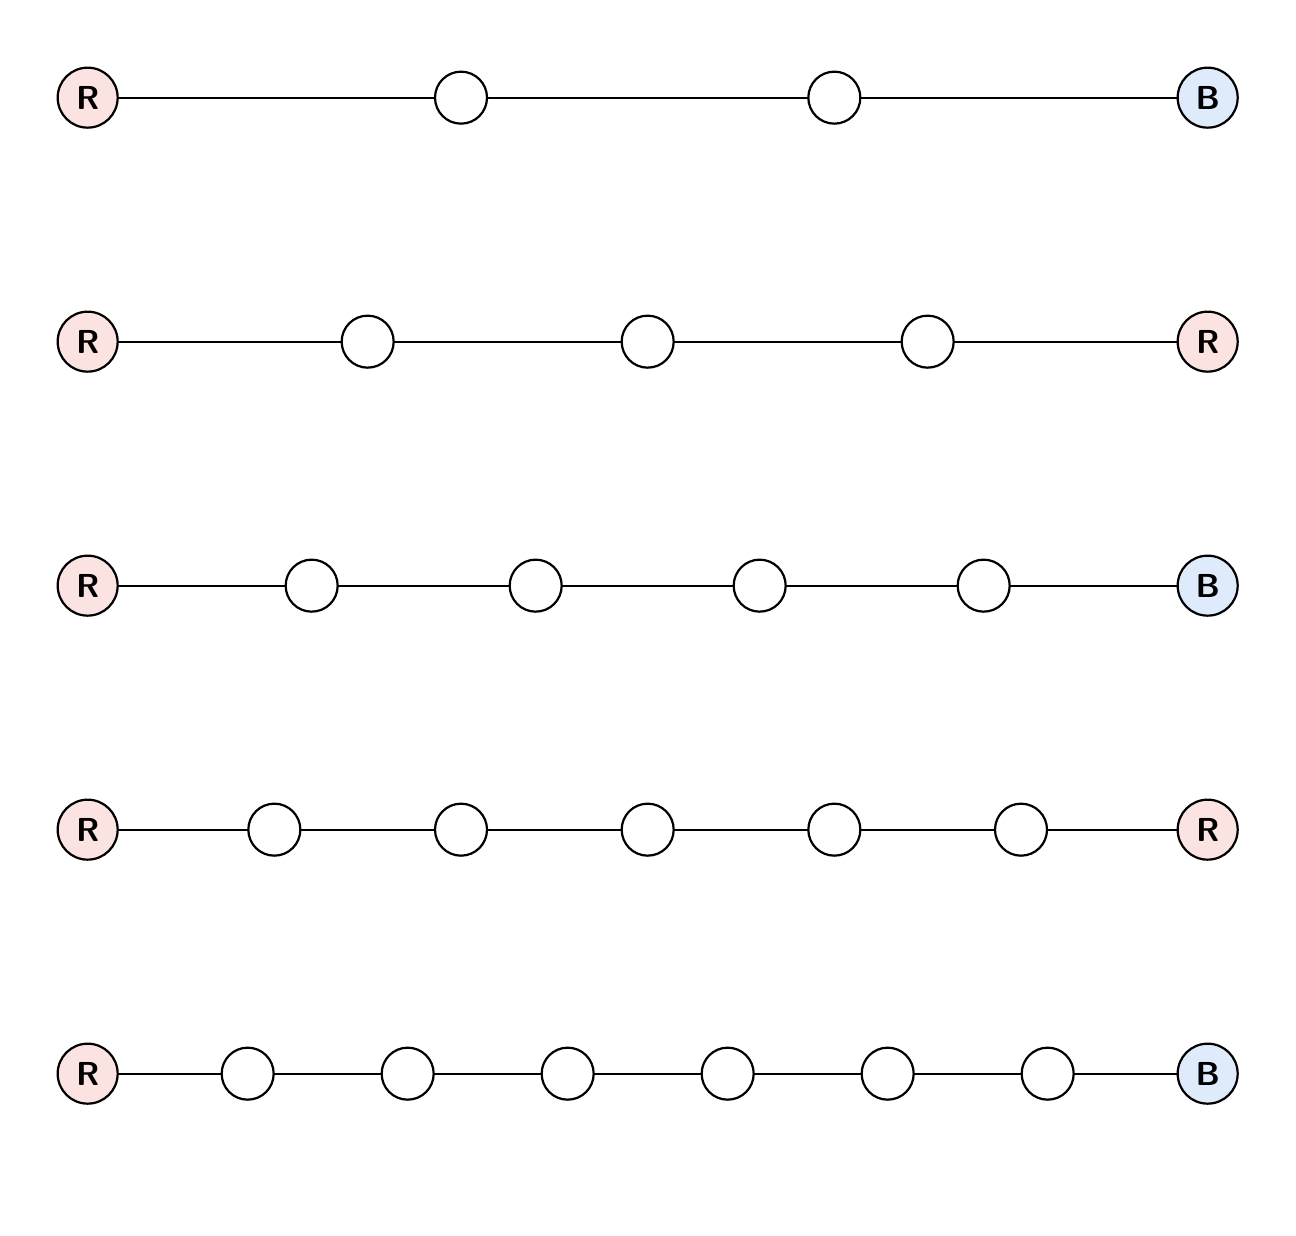
\begin{tikzpicture}[x=1in,y=1in,line cap=round]
\path[use as bounding box] (-0.3,-0.25) rectangle (5.9,5.65);
\draw[line width=0.8pt] (0,5.3000) -- (5.6,5.3000);
\node[circle,draw,line width=0.8pt,fill=Rfill,minimum size=0.30in,inner sep=0pt,font=\sffamily\bfseries\fontsize{11.5}{12}\selectfont] at (0.0000,5.3000) {R};
\draw[line width=0.8pt,fill=white] (1.8667,5.3000) circle[radius=0.13in];
\draw[line width=0.8pt,fill=white] (3.7333,5.3000) circle[radius=0.13in];
\node[circle,draw,line width=0.8pt,fill=Bfill,minimum size=0.30in,inner sep=0pt,font=\sffamily\bfseries\fontsize{11.5}{12}\selectfont] at (5.6000,5.3000) {B};
\draw[line width=0.8pt] (0,4.0800) -- (5.6,4.0800);
\node[circle,draw,line width=0.8pt,fill=Rfill,minimum size=0.30in,inner sep=0pt,font=\sffamily\bfseries\fontsize{11.5}{12}\selectfont] at (0.0000,4.0800) {R};
\draw[line width=0.8pt,fill=white] (1.4000,4.0800) circle[radius=0.13in];
\draw[line width=0.8pt,fill=white] (2.8000,4.0800) circle[radius=0.13in];
\draw[line width=0.8pt,fill=white] (4.2000,4.0800) circle[radius=0.13in];
\node[circle,draw,line width=0.8pt,fill=Rfill,minimum size=0.30in,inner sep=0pt,font=\sffamily\bfseries\fontsize{11.5}{12}\selectfont] at (5.6000,4.0800) {R};
\draw[line width=0.8pt] (0,2.8600) -- (5.6,2.8600);
\node[circle,draw,line width=0.8pt,fill=Rfill,minimum size=0.30in,inner sep=0pt,font=\sffamily\bfseries\fontsize{11.5}{12}\selectfont] at (0.0000,2.8600) {R};
\draw[line width=0.8pt,fill=white] (1.1200,2.8600) circle[radius=0.13in];
\draw[line width=0.8pt,fill=white] (2.2400,2.8600) circle[radius=0.13in];
\draw[line width=0.8pt,fill=white] (3.3600,2.8600) circle[radius=0.13in];
\draw[line width=0.8pt,fill=white] (4.4800,2.8600) circle[radius=0.13in];
\node[circle,draw,line width=0.8pt,fill=Bfill,minimum size=0.30in,inner sep=0pt,font=\sffamily\bfseries\fontsize{11.5}{12}\selectfont] at (5.6000,2.8600) {B};
\draw[line width=0.8pt] (0,1.6400) -- (5.6,1.6400);
\node[circle,draw,line width=0.8pt,fill=Rfill,minimum size=0.30in,inner sep=0pt,font=\sffamily\bfseries\fontsize{11.5}{12}\selectfont] at (0.0000,1.6400) {R};
\draw[line width=0.8pt,fill=white] (0.9333,1.6400) circle[radius=0.13in];
\draw[line width=0.8pt,fill=white] (1.8667,1.6400) circle[radius=0.13in];
\draw[line width=0.8pt,fill=white] (2.8000,1.6400) circle[radius=0.13in];
\draw[line width=0.8pt,fill=white] (3.7333,1.6400) circle[radius=0.13in];
\draw[line width=0.8pt,fill=white] (4.6667,1.6400) circle[radius=0.13in];
\node[circle,draw,line width=0.8pt,fill=Rfill,minimum size=0.30in,inner sep=0pt,font=\sffamily\bfseries\fontsize{11.5}{12}\selectfont] at (5.6000,1.6400) {R};
\draw[line width=0.8pt] (0,0.4200) -- (5.6,0.4200);
\node[circle,draw,line width=0.8pt,fill=Rfill,minimum size=0.30in,inner sep=0pt,font=\sffamily\bfseries\fontsize{11.5}{12}\selectfont] at (0.0000,0.4200) {R};
\draw[line width=0.8pt,fill=white] (0.8000,0.4200) circle[radius=0.13in];
\draw[line width=0.8pt,fill=white] (1.6000,0.4200) circle[radius=0.13in];
\draw[line width=0.8pt,fill=white] (2.4000,0.4200) circle[radius=0.13in];
\draw[line width=0.8pt,fill=white] (3.2000,0.4200) circle[radius=0.13in];
\draw[line width=0.8pt,fill=white] (4.0000,0.4200) circle[radius=0.13in];
\draw[line width=0.8pt,fill=white] (4.8000,0.4200) circle[radius=0.13in];
\node[circle,draw,line width=0.8pt,fill=Bfill,minimum size=0.30in,inner sep=0pt,font=\sffamily\bfseries\fontsize{11.5}{12}\selectfont] at (5.6000,0.4200) {B};
\end{tikzpicture}
\end{center}
\newpage
\textbf{Problem 5:} Must the number of little triangles with R, B, and Y be odd? Explain your answer for every filling allowed by the side rules, on this board and on any division into little triangles that meet only at corners or along whole edges.\par\vspace{0.16in}
\begin{center}
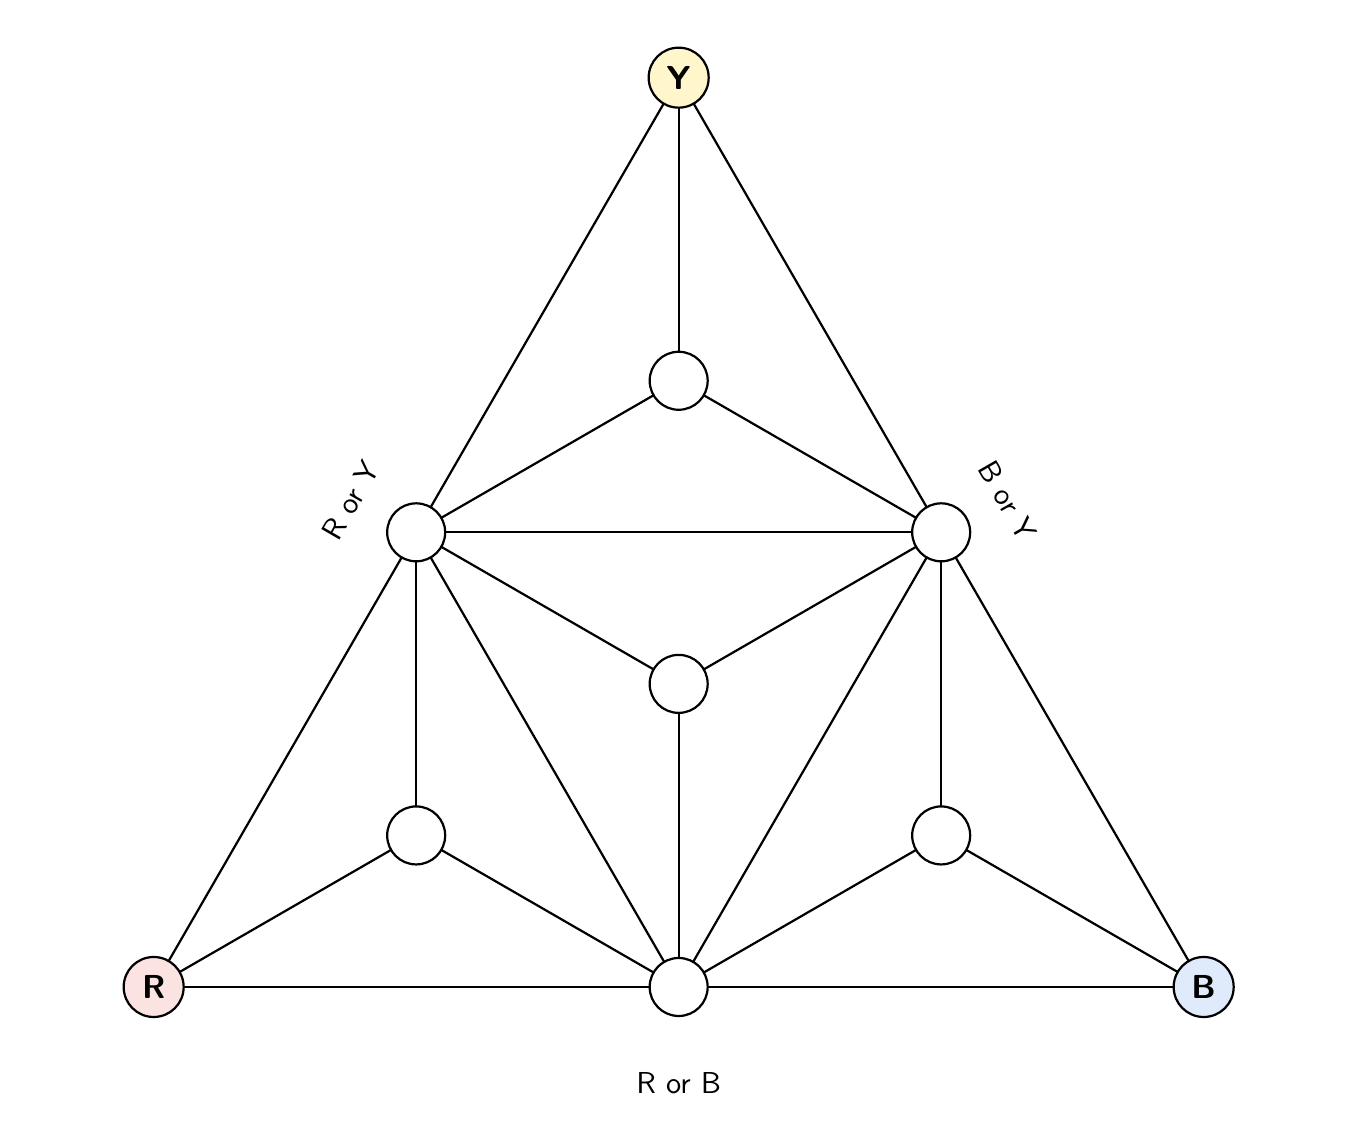
\begin{tikzpicture}[x=1in,y=1in,line cap=round,line join=round]
\path[use as bounding box] (-0.63,-0.64) rectangle (5.8800,4.7966);
\draw[line width=0.8pt] (0.0000,0.0000) -- (1.3125,2.2733);
\draw[line width=0.8pt] (0.0000,0.0000) -- (2.6250,0.0000);
\draw[line width=0.8pt] (0.0000,0.0000) -- (1.3125,0.7578);
\draw[line width=0.8pt] (1.3125,2.2733) -- (2.6250,4.5466);
\draw[line width=0.8pt] (1.3125,2.2733) -- (2.6250,0.0000);
\draw[line width=0.8pt] (1.3125,2.2733) -- (3.9375,2.2733);
\draw[line width=0.8pt] (1.3125,2.2733) -- (1.3125,0.7578);
\draw[line width=0.8pt] (1.3125,2.2733) -- (2.6250,1.5155);
\draw[line width=0.8pt] (1.3125,2.2733) -- (2.6250,3.0311);
\draw[line width=0.8pt] (2.6250,4.5466) -- (3.9375,2.2733);
\draw[line width=0.8pt] (2.6250,4.5466) -- (2.6250,3.0311);
\draw[line width=0.8pt] (2.6250,0.0000) -- (3.9375,2.2733);
\draw[line width=0.8pt] (2.6250,0.0000) -- (5.2500,0.0000);
\draw[line width=0.8pt] (2.6250,0.0000) -- (1.3125,0.7578);
\draw[line width=0.8pt] (2.6250,0.0000) -- (2.6250,1.5155);
\draw[line width=0.8pt] (2.6250,0.0000) -- (3.9375,0.7578);
\draw[line width=0.8pt] (3.9375,2.2733) -- (5.2500,0.0000);
\draw[line width=0.8pt] (3.9375,2.2733) -- (2.6250,1.5155);
\draw[line width=0.8pt] (3.9375,2.2733) -- (3.9375,0.7578);
\draw[line width=0.8pt] (3.9375,2.2733) -- (2.6250,3.0311);
\draw[line width=0.8pt] (5.2500,0.0000) -- (3.9375,0.7578);
\node[circle,draw,line width=0.8pt,fill=Rfill,minimum size=0.30in,inner sep=0pt,font=\sffamily\bfseries\fontsize{11.5}{12}\selectfont] at (0.0000,0.0000) {R};
\draw[line width=0.8pt,fill=white] (2.6250,0.0000) circle[radius=0.145in];
\node[circle,draw,line width=0.8pt,fill=Bfill,minimum size=0.30in,inner sep=0pt,font=\sffamily\bfseries\fontsize{11.5}{12}\selectfont] at (5.2500,0.0000) {B};
\draw[line width=0.8pt,fill=white] (1.3125,2.2733) circle[radius=0.145in];
\draw[line width=0.8pt,fill=white] (3.9375,2.2733) circle[radius=0.145in];
\node[circle,draw,line width=0.8pt,fill=Yfill,minimum size=0.30in,inner sep=0pt,font=\sffamily\bfseries\fontsize{11.5}{12}\selectfont] at (2.6250,4.5466) {Y};
\draw[line width=0.8pt,fill=white] (1.3125,0.7578) circle[radius=0.145in];
\draw[line width=0.8pt,fill=white] (2.6250,1.5155) circle[radius=0.145in];
\draw[line width=0.8pt,fill=white] (3.9375,0.7578) circle[radius=0.145in];
\draw[line width=0.8pt,fill=white] (2.6250,3.0311) circle[radius=0.145in];
\node[rotate=60,font=\sffamily\fontsize{11}{12}\selectfont] at (0.9825,2.4333) {R or Y};
\node[rotate=-60,font=\sffamily\fontsize{11}{12}\selectfont] at (4.2675,2.4333) {B or Y};
\node[font=\sffamily\fontsize{11}{12}\selectfont] at (2.6250,-0.48) {R or B};
\end{tikzpicture}
\end{center}
\newpage
\textbf{Problem 6:} The starred dot may now use R, B, or Y. All other side rules still hold. Find a filling with no little triangle that has R, B, and Y. Explain why this does not contradict your answer to Problem 5.\par\vspace{0.16in}
\begin{center}
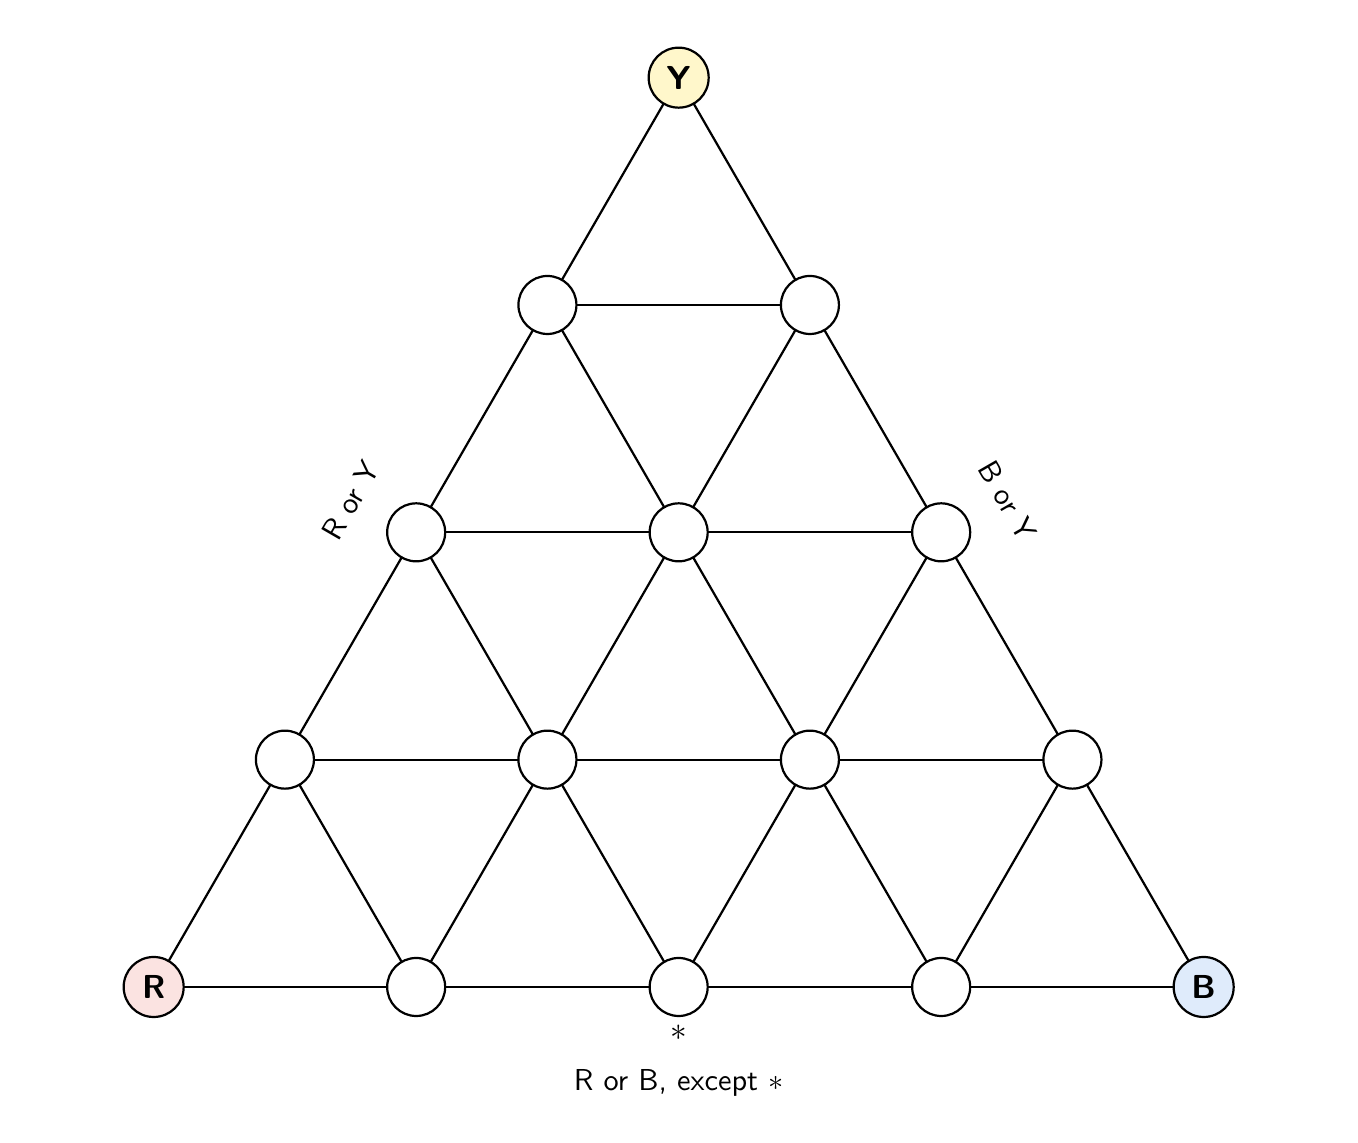
\begin{tikzpicture}[x=1in,y=1in,line cap=round,line join=round]
\path[use as bounding box] (-0.63,-0.64) rectangle (5.8800,4.7966);
\draw[line width=0.8pt] (0.0000,0.0000) -- (0.6562,1.1367);
\draw[line width=0.8pt] (0.0000,0.0000) -- (1.3125,0.0000);
\draw[line width=0.8pt] (0.6562,1.1367) -- (1.3125,2.2733);
\draw[line width=0.8pt] (0.6562,1.1367) -- (1.3125,0.0000);
\draw[line width=0.8pt] (0.6562,1.1367) -- (1.9688,1.1367);
\draw[line width=0.8pt] (1.3125,2.2733) -- (1.9688,3.4100);
\draw[line width=0.8pt] (1.3125,2.2733) -- (1.9688,1.1367);
\draw[line width=0.8pt] (1.3125,2.2733) -- (2.6250,2.2733);
\draw[line width=0.8pt] (1.9688,3.4100) -- (2.6250,4.5466);
\draw[line width=0.8pt] (1.9688,3.4100) -- (2.6250,2.2733);
\draw[line width=0.8pt] (1.9688,3.4100) -- (3.2812,3.4100);
\draw[line width=0.8pt] (2.6250,4.5466) -- (3.2812,3.4100);
\draw[line width=0.8pt] (1.3125,0.0000) -- (1.9688,1.1367);
\draw[line width=0.8pt] (1.3125,0.0000) -- (2.6250,0.0000);
\draw[line width=0.8pt] (1.9688,1.1367) -- (2.6250,2.2733);
\draw[line width=0.8pt] (1.9688,1.1367) -- (2.6250,0.0000);
\draw[line width=0.8pt] (1.9688,1.1367) -- (3.2812,1.1367);
\draw[line width=0.8pt] (2.6250,2.2733) -- (3.2812,3.4100);
\draw[line width=0.8pt] (2.6250,2.2733) -- (3.2812,1.1367);
\draw[line width=0.8pt] (2.6250,2.2733) -- (3.9375,2.2733);
\draw[line width=0.8pt] (3.2812,3.4100) -- (3.9375,2.2733);
\draw[line width=0.8pt] (2.6250,0.0000) -- (3.2812,1.1367);
\draw[line width=0.8pt] (2.6250,0.0000) -- (3.9375,0.0000);
\draw[line width=0.8pt] (3.2812,1.1367) -- (3.9375,2.2733);
\draw[line width=0.8pt] (3.2812,1.1367) -- (3.9375,0.0000);
\draw[line width=0.8pt] (3.2812,1.1367) -- (4.5938,1.1367);
\draw[line width=0.8pt] (3.9375,2.2733) -- (4.5938,1.1367);
\draw[line width=0.8pt] (3.9375,0.0000) -- (4.5938,1.1367);
\draw[line width=0.8pt] (3.9375,0.0000) -- (5.2500,0.0000);
\draw[line width=0.8pt] (4.5938,1.1367) -- (5.2500,0.0000);
\node[circle,draw,line width=0.8pt,fill=Rfill,minimum size=0.30in,inner sep=0pt,font=\sffamily\bfseries\fontsize{11.5}{12}\selectfont] at (0.0000,0.0000) {R};
\draw[line width=0.8pt,fill=white] (1.3125,0.0000) circle[radius=0.145in];
\draw[line width=0.8pt,fill=white] (2.6250,0.0000) circle[radius=0.145in];
\draw[line width=0.8pt,fill=white] (3.9375,0.0000) circle[radius=0.145in];
\node[circle,draw,line width=0.8pt,fill=Bfill,minimum size=0.30in,inner sep=0pt,font=\sffamily\bfseries\fontsize{11.5}{12}\selectfont] at (5.2500,0.0000) {B};
\draw[line width=0.8pt,fill=white] (0.6562,1.1367) circle[radius=0.145in];
\draw[line width=0.8pt,fill=white] (1.9688,1.1367) circle[radius=0.145in];
\draw[line width=0.8pt,fill=white] (3.2812,1.1367) circle[radius=0.145in];
\draw[line width=0.8pt,fill=white] (4.5938,1.1367) circle[radius=0.145in];
\draw[line width=0.8pt,fill=white] (1.3125,2.2733) circle[radius=0.145in];
\draw[line width=0.8pt,fill=white] (2.6250,2.2733) circle[radius=0.145in];
\draw[line width=0.8pt,fill=white] (3.9375,2.2733) circle[radius=0.145in];
\draw[line width=0.8pt,fill=white] (1.9688,3.4100) circle[radius=0.145in];
\draw[line width=0.8pt,fill=white] (3.2812,3.4100) circle[radius=0.145in];
\node[circle,draw,line width=0.8pt,fill=Yfill,minimum size=0.30in,inner sep=0pt,font=\sffamily\bfseries\fontsize{11.5}{12}\selectfont] at (2.6250,4.5466) {Y};
\node[rotate=60,font=\sffamily\fontsize{11}{12}\selectfont] at (0.9825,2.4333) {R or Y};
\node[rotate=-60,font=\sffamily\fontsize{11}{12}\selectfont] at (4.2675,2.4333) {B or Y};
\node[font=\sffamily\fontsize{11}{12}\selectfont] at (2.6250,-0.48) {R or B, except $*$};
\node[font=\large] at (2.6250,-0.23) {$*$};
\end{tikzpicture}
\end{center}
\end{document}
